\documentclass{article}
\usepackage[T1]{fontenc}
\usepackage{helvet}
\renewcommand{\familydefault}{\sfdefault}
\usepackage{graphicx}
\usepackage{amsmath,amsthm,amssymb,latexsym}
\usepackage{enumerate}
\usepackage{hyperref}
\usepackage{url}

\newcommand{\no}{\noindent}
\newcommand{\bn}{\bigskip\noindent}
\newcommand{\sn}{\smallskip\noindent}
\newcommand{\mn}{\medskip\noindent}

\begin{document}
\begin{center}
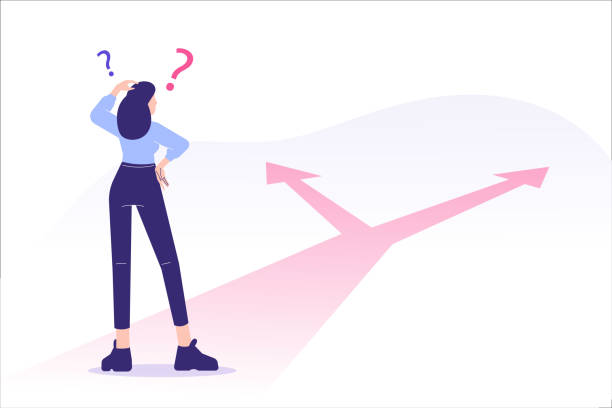
\includegraphics[scale=2]{fig/probabilistic-paths.jpg}
\end{center}

\mn
{\huge\bf Probabilistic Pathways: Modeling}

\bn
{\huge\bf Human Navigation Decisions in}

\bn
{\huge\bf Urban Environments}

\bn

\section*{Is There a Probability of Turning Right or Left at the First Intersection When Walking Down a Road in a Town?}


When you walk down the road in a town and approach an intersection, there is indeed a {\bf probability}  associated with whether you will turn right or turn left. These probabilities can be thought of as representing the uncertainty in your decision-making process at that moment.



\subsection*{How This Relates to the Whole-in-One Framework?}

This scenario can be modeled using the {\bf Whole-in-One Framework} , as it captures probabilistic decision-making based on inputs, biases, {\bf divine influence} , and contextual factors. Let's break it down:

\begin{enumerate}[1.]
\item  Inputs ($x_j$):  

$\bullet$  Your inputs in this scenario could include:

\begin{itemize}
\item[$\circ$]  The layout of the road (e.g., whether one path looks more appealing).
\item[$\circ$]  Traffic conditions.
\item[$\circ$]  Your destination or goal.
\end{itemize}


\item   Weights ($w_{ij}$):

\begin{itemize}  
\item Different inputs have varying importance, which is reflected in their {\bf weights} . For example:

\begin{itemize}
\item[$\circ$]   If your destination is to the right, the "destination" input will have a higher weight for turning right.
\item[$\circ$]  If you see something visually attractive on the left (e.g., a shop or park), it might increase the weight for turning left.
\end{itemize}
\end{itemize}

\item   Bias ($b_i$):

\begin{itemize}  
\item   Your bias reflects personal tendencies or habits. For example:

\begin{itemize}
\item[$\circ$]  You might have a habit of favoring one direction (e.g., always turning right first).
\item[$\circ$]  A subconscious preference might influence the decision (e.g., avoiding noisy or crowded areas).
\end{itemize}
\end{itemize}

\item   Divine Influence ($G_{ij}$):

\begin{itemize}
\item In addition to rational and emotional factors, there may be a subtle influence beyond human control.
\item {\bf Intuition or ``inner guidance''} : A feeling that nudges you toward a certain direction.
\item {\bf Unexpected encounters} : You take an unexpected turn and meet someone important---was this random or divinely orchestrated?
\item {\bf Faith and decision-making} : Some paths are chosen based on a sense of purpose or spiritual conviction.
\end{itemize}

The equation integrating divine influence becomes:

$$
\sigma \left(\sum_{j} (w_{ij} + G_{ij}) \cdot x_j + b_i \right) = D_i
$$

where {\bf $G_{ij}$ represents divine influence} , a factor that subtly guides decision-making beyond immediate rational considerations.

\item   Decision Probability ($D_i$):

\begin{itemize}
\item  The final probability of each decision (turning right or left) is computed using the sigmoid function.
\item  This probability integrates {\bf rational factors, personal biases, and divine adjustments} , assigning a {\bf probabilistic value}  to each possible decision.
   
\end{itemize}
\end{enumerate}


\subsection*{What Influences the Probabilities?}

Your decision probabilities are influenced by various {\bf contextual and unseen factors} :

\begin{itemize}
\item   {\bf Current Goal:}  If you have a specific destination in mind, the probability will be heavily weighted toward the direction of that destination.
\item   {\bf External Environment:}  A crowded street, a nice café, or a beautiful park can shift your decision probabilities.
\item    {\bf Random Factors:}  Even with all the inputs and weights, there's still an element of randomness in human decision-making that adds uncertainty.
\item    {\bf Divine Guidance:}  A seemingly random decision could lead to an outcome of deeper significance, aligning with a higher purpose.
\end{itemize}


\subsection*{Why Is This Important?}

This example highlights the {\bf core insight}  of the Whole-in-One Framework: {\bf Human decision-making is inherently probabilistic, influenced by raw information, experience, emotion, and divine guidance.} 

\begin{itemize}
\item   In real-world scenarios, we don't always have complete certainty about our choices.
\item  The framework acknowledges this by assigning {\bf probabilities}  to decisions rather than deterministic outcomes.
\item   Divine influence adds a {\bf higher-order adjustment}, which may shape significant life events beyond what appears as mere chance.
\end{itemize}


\subsection*{Broader Applications}

The same probabilistic approach can be applied to:

\begin{itemize}
\item   {\bf Traffic flow models:}  Predicting how pedestrians or drivers navigate urban environments.
\item   {\bf Behavioral psychology:}  Understanding how humans make everyday decisions.
\item  {\bf AI and robotics:}  Designing systems that mimic human-like decision-making under uncertainty.
\item   {\bf Faith and purpose:}  Exploring how unseen influences may guide human choices.
\end{itemize}

\subsection*{Conclusion: A Microcosm of the Whole-in-One Framework}

This simple act of {\bf choosing between right and left}  is a small-scale representation of {\bf how all human decisions operate} ---through {\bf a balance of information, habit, uncertainty, and guidance} .  

The Whole-in-One Framework provides a lens to understand {\bf not only financial markets but also the way we navigate life itself} .

\end{document}

\begin{itemize}
\item  
\item 
\end{itemize}

